
	\subsubsection{Use-Case Instance - ucisuScenarioPresentation:suScenarioPresentation}
	
	Represents the instance of the three combined variants.		  
	\begin{operationmodel}
	\addheading{summary Use-Case Instance}
	\adddoublerow{Instantiated Use Case}{suScenarioPresentation}
	\adddoublerow{Instance ID}{ucisuScenarioPresentation}
	
	\end{operationmodel} 

	
	Figure \ref{fig:lu.uni.lassy.excalibur.MyCrash.G02-RE-UC-uci-ucisuScenarioPresentation}
	Present the collaboration of the three variants.
	
	\begin{figure}[htbp]
	\begin{center}
	
	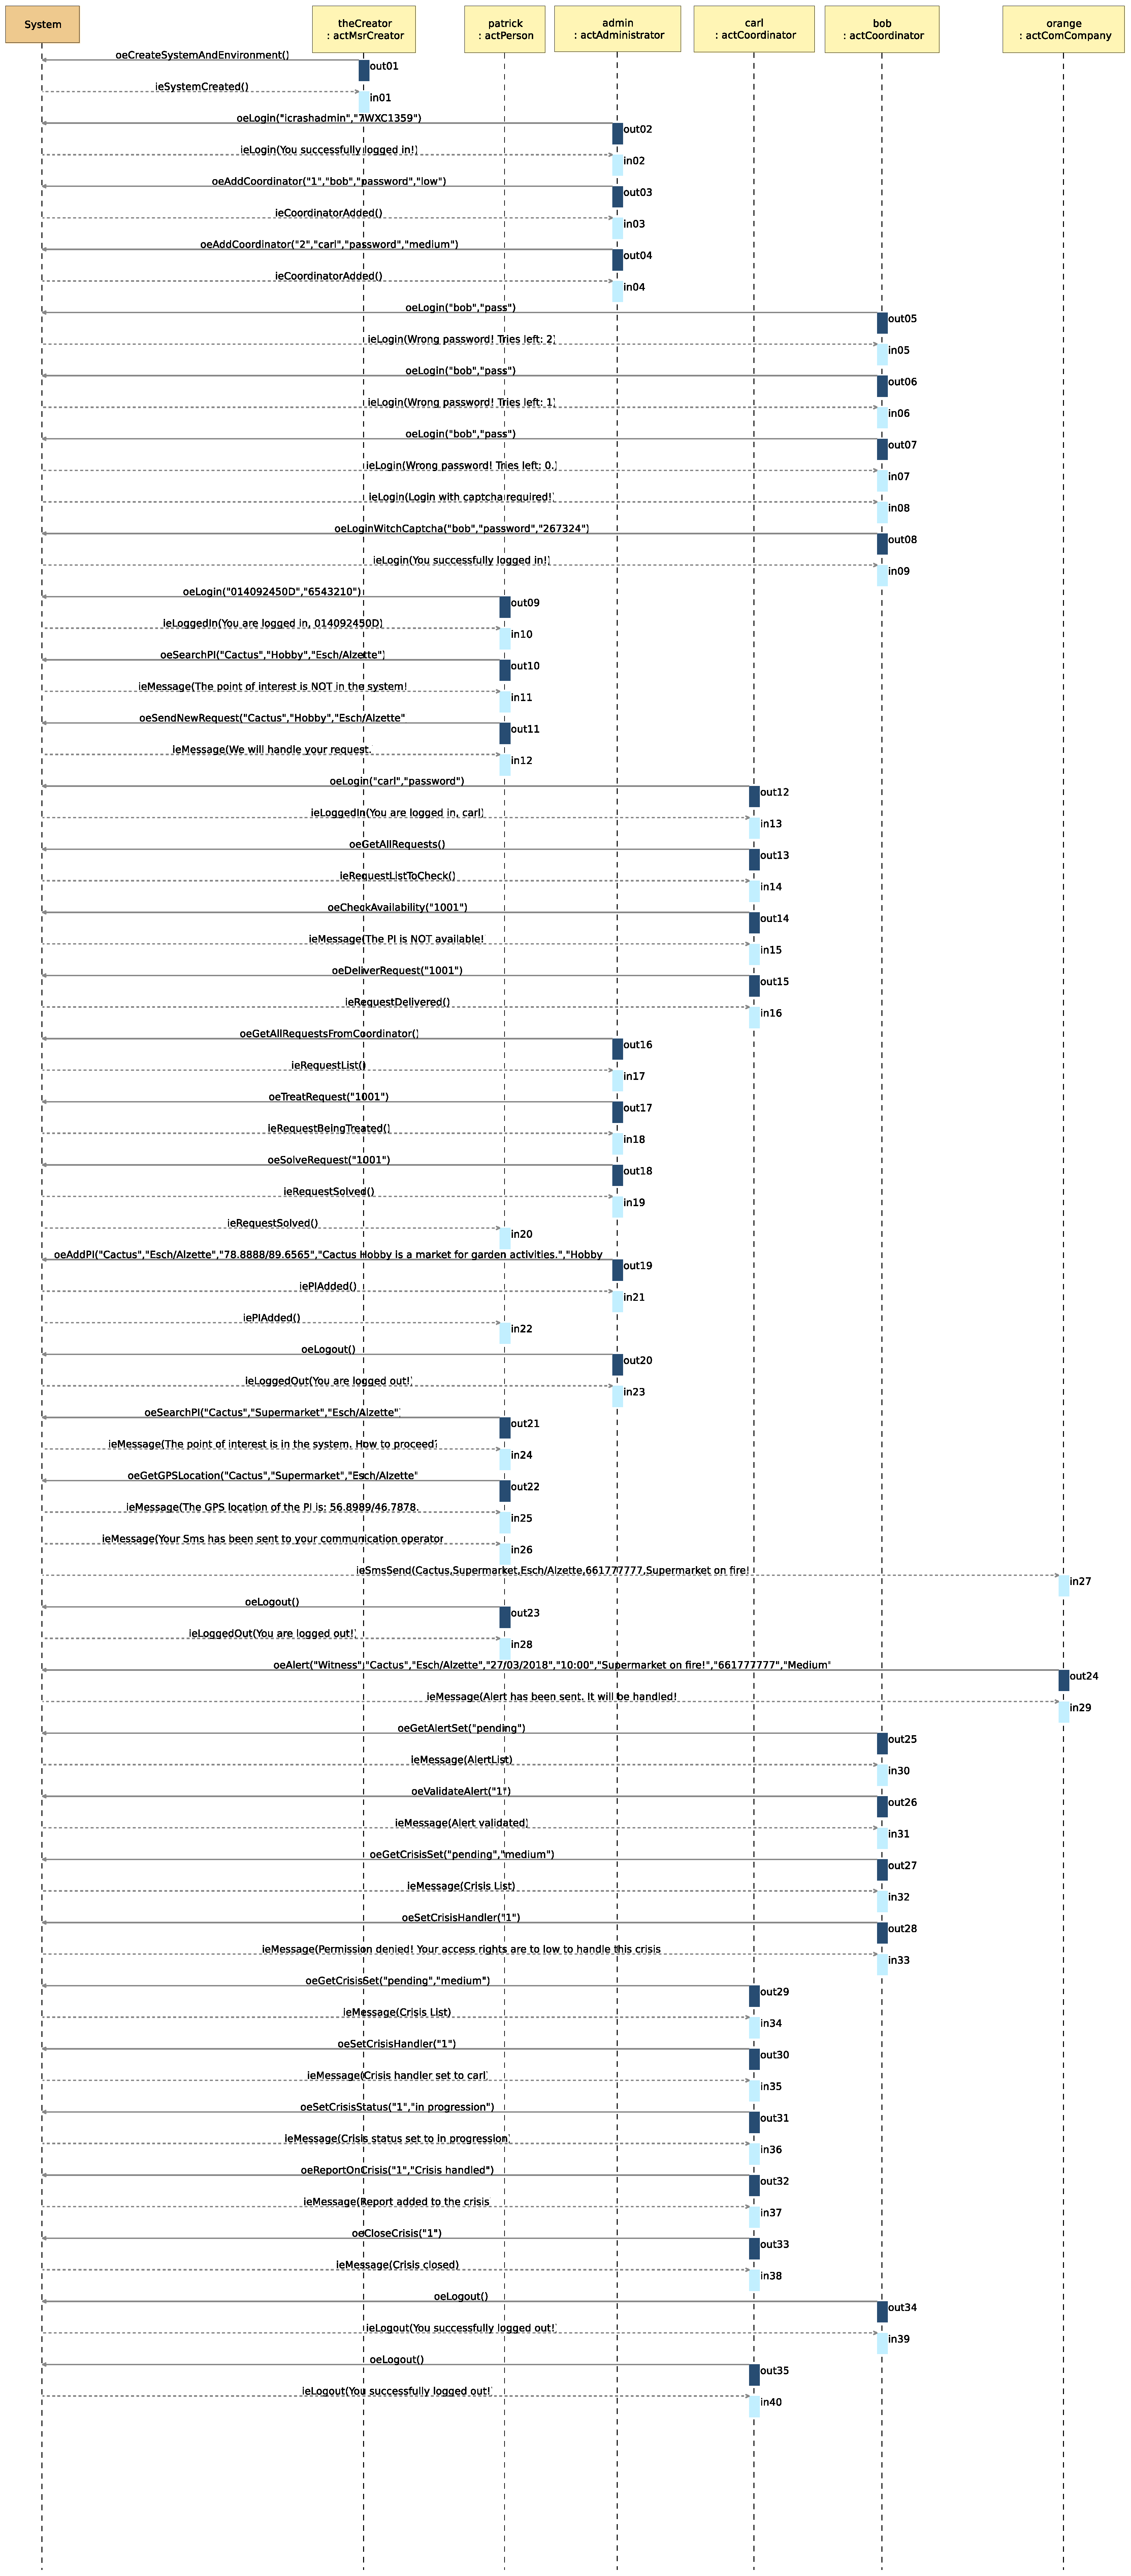
\includegraphics[
	angle=0
	,width=1.0\textwidth
	]{./images-report-gen/usecase-model/summary/uci-ucisuScenarioPresentation.eps}
	\end{center}
	\caption[lu.uni.lassy.excalibur.MyCrash.G02 Sequence Diagram: uci-ucisuScenarioPresentation]{uci-suScenarioPresentation-uciSceanrioPresentation use case instance sequence diagram}
	\label{fig:lu.uni.lassy.excalibur.MyCrash.G02-RE-UC-uci-ucisuScenarioPresentation}
	\end{figure}
	\vspace{0.5cm}
